% This template was initially provided by Dulip Withanage.
% Modifications for the database systems research group
% were made by Conny Junghans,  Jannik Strtgen and Michael Gertz

\documentclass[
     12pt,         % font size
     a4paper,      % paper format
     BCOR=10mm,version=first,     % binding correction
     DIV=14,version=first,        % stripe size for margin calculation
%     liststotoc,   % table listing in toc
%     bibtotoc,     % bibliography in toc
%     idxtotoc,     % index in toc
%     parskip       % paragraph skip instad of paragraph indent
     ]{scrreprt}

%%%%%%%%%%%%%%%%%%%%%%%%%%%%%%%%%%%%%%%%%%%%%%%%%%%%%%%%%%%%

% PACKAGES:

% Use German :
\usepackage[english]{babel}
% Input and font encoding
\usepackage[utf8]{inputenc}
\usepackage[T1]{fontenc}
% Index-generation
\usepackage{makeidx}
% Einbinden von URLs:
\usepackage{url}
% Special \LaTex symbols (e.g. \BibTeX):
%\usepackage{doc}
% Include Graphic-files:
\usepackage{graphicx}
% Include doc++ generated tex-files:
%\usepackage{docxx}
% Include PDF links
%\usepackage[pdftex, bookmarks=true]{hyperref}
\usepackage{csquotes}
\usepackage{color, colortbl, tabularx, ragged2e}
\definecolor{LightCyan}{rgb}{0.88,1,1}
\newcolumntype{C}{>{\raggedright\arraybackslash}X} % centered "X" column
% Fuer anderthalbzeiligen Textsatz
\usepackage{setspace}
\usepackage{multirow}
\usepackage{longtable}
\usepackage{float}

\usepackage{subfiles} % Best loaded last in the preamble

% hyperrefs in the documents
\usepackage[bookmarks=true,colorlinks,pdfpagelabels,pdfstartview = FitH,bookmarksopen = true,bookmarksnumbered = true,linkcolor = black,plainpages = false,hypertexnames = false,citecolor = black,urlcolor=black]{hyperref} 
%\usepackage{hyperref}


%%%%%%%%%%%%%%%%%%%%%%%%%%%%%%%%%%%%%%%%%%%%%%%%%%%%%%%%%%%%

% OTHER SETTINGS:

% Pagestyle:
\pagestyle{headings}

% Choose language
\newcommand{\setlang}[1]{\selectlanguage{#1}\nonfrenchspacing}

\usepackage{biblatex}
\addbibresource{references.bib}

\begin{document}

% TITLE:
\pagenumbering{roman}
\begin{titlepage}
     \vspace*{1cm}
     \begin{center}
          \vspace*{3cm}
          \textbf
          {
               \Large University of Heidelberg\\
               \smallskip
               \Large Institute for Computer Science\\
               \smallskip
               \Large Working group database systems\\
               \smallskip
          }

          \vspace{3cm}

          \textbf{\large Bachelor thesis}

          \vspace{0.5\baselineskip}
          {
               \huge
               \textbf{Integrating Identity Management Providers based on Online Zugangs Gesetz}
          }

     \end{center}

     \vfill
     {
          \large
          \begin{tabular}[l]{ll}
               Name:                 & Jonas Gann              \\
               Matriculation number: & 3367576                 \\
               Supervisor:           & Prof. Dr. Michael Gertz \\
               Date of submission:   & \today
          \end{tabular}
     }

\end{titlepage}

\onehalfspacing

\thispagestyle{empty}

\vspace*{100pt}
\noindent
I assure that I have written this bachelor thesis on my own and only used the specified sources and resources and that I followed the principles and recommendations "Responsibility in Science" of the University of Heidelberg.

\vspace*{50pt}
\noindent

\underline{\phantom{mmmmmmmmmmmmmmmmmmmm}}

\medskip
\noindent
Date of Submission: \today
\newpage

\chapter*{Zusammenfassung}

\newpage

\chapter*{Abstract}

\newpage

\tableofcontents
\cleardoublepage
\pagenumbering{arabic}

\chapter{Introduction}

\section{Context}

\subfile{sections/1-context}

\section{Objective}

\subfile{sections/2-objective}

\section{Structure of Work}

\subfile{sections/3-structure_of_work}

\chapter{Background and Related Work}

\section{Terminology}

\subfile{sections/4-terminology}

\section{Online Access Law (OZG)}

\subfile{sections/5-online_access_law}

\chapter{Identity Management}

\section{Functional Requirement Analysis}

\subfile{sections/6-requirement_analysis}

\section{IMP System Proposal}

\subfile{sections/7-imp_system_proposal}

\chapter{Minimal Integration Architecture}

The goal of the integration architecture is to make as many functionalities required for the basic OZG use case available through the IMP client as possible. As described in chapter 2.3, the steps of the basic OZG use case are:
\begin{enumerate}
    \item{Create User Profile}
    \item{Login to User Profile}
    \item{Selection of Administrative Service}
    \item{Filling in Application}
    \item{Submission of Application}
    \item{Reception of Application by Administration Portal}
    \item{Submission of Application to Data-Exchange Platform}
    \item{Management of Applications}
    \item{Communication}
\end{enumerate}

To enable service providers a quick introduction of IMP systems into their system architecture, this integration architecture describes a minimally invasive integration. After deployment of this integration architecture, all OZG services are still usable as before but can be enhanced by IMP solutions. For this integration to be minimally invasive, only one connector exists and integrates only with the administration portal. No other OZG system component is modified or directly accessed.

The goal of the integration is to enhance each step of the basic OZG use case through integration with IMP solutions. Therefore in the overview section, for each step, possible integration's of OZG systems are evaluated. The following sections contain more detailed descriptions of the selected integration strategies.

\begin{figure}[h]
    \centering
    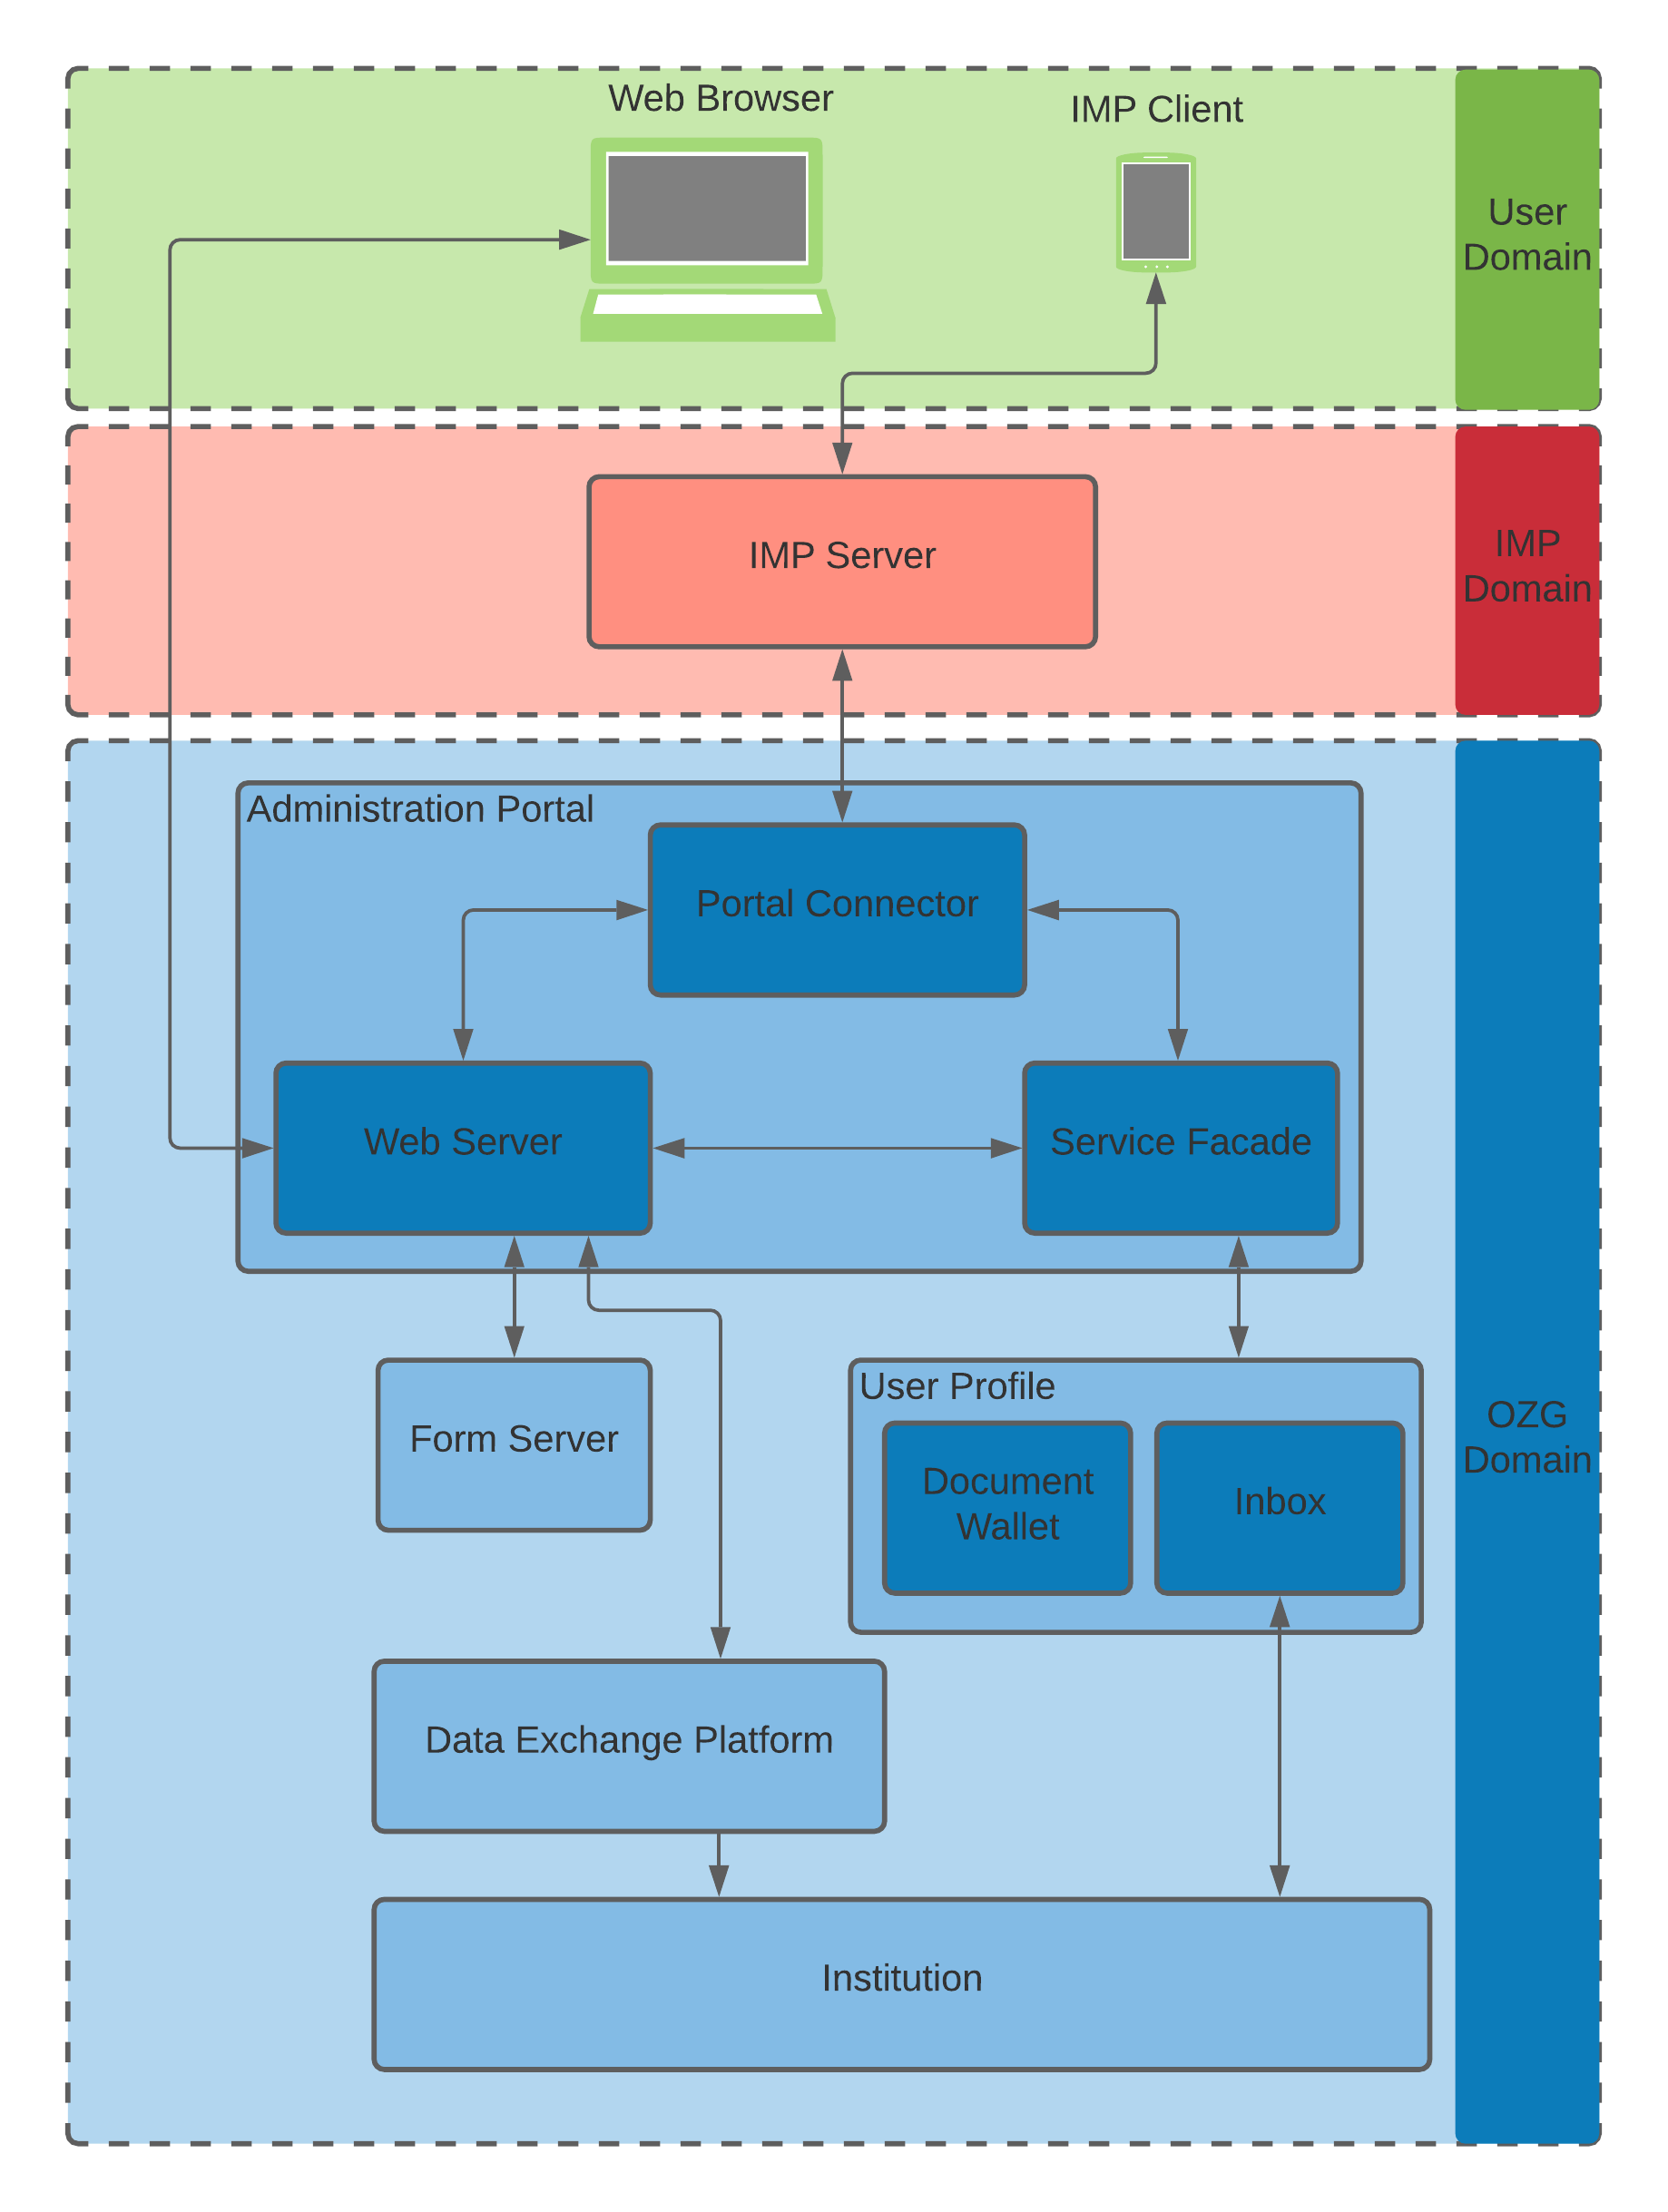
\includegraphics[scale=0.15]{Diagrams/Integration Architecture 1/Overview.png}
\end{figure}

\section{IMP Solution Integration}

\subfile{sections/8-imp_solution_integration}

\section{Technological Integration}

\subfile{sections/9-technological_integration}


\chapter{Advanced Integration Architecture}

The goal of this integration architecture is to make as much functionalities required for the basic OZG use case available through the IMP client. Now, the OZG user profiles are replaced with IMP identities and the integration architecture integrates with any system component necessary.

\begin{figure}[h]
    \centering
    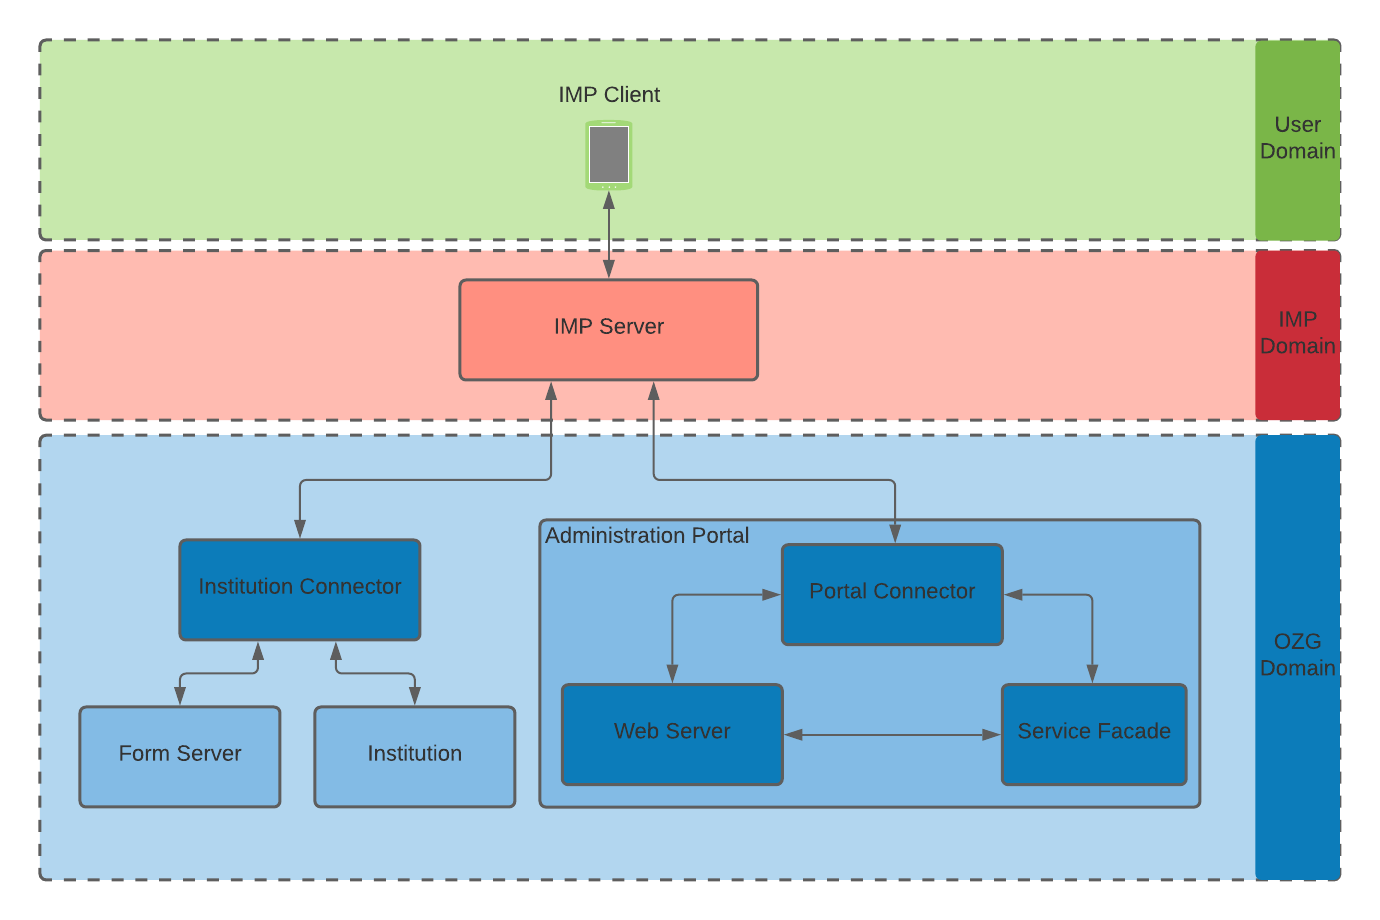
\includegraphics[scale=0.15]{Diagrams/Integration Architecture 2/Overview.png}
\end{figure}

\section{IMP Solution Integration}

\chapter{Solution Evaluation}

\section{Conclusion}

\chapter{Outlook: Advanced IMP Integration}


\printbibliography


\end{document}
